\documentclass[margin=.2cm]{article}

%% https://tex.stackexchange.com/questions/500427/drawing-an-accurate-guitar-fretboard-with-tikz

\usepackage{tikz}
\usetikzlibrary{calc,arrows}

\tikzset{zbar/.style={
  shorten >=-3,
  shorten <=-3,
  line width=6,
  round cap-round cap}}
\tikzset{znode/.style={
  white,
  draw=black,
  circle,
  fill=black,
  scale=.4,
  inner sep=1pt,
  minimum size=1.7em}}
\tikzset{zroot/.style={
  black,
  draw=black,
  circle,
  fill=white,
  scale=.4,
  inner sep=1pt,
  minimum size=1.7em}}

\begin{document}

\centering

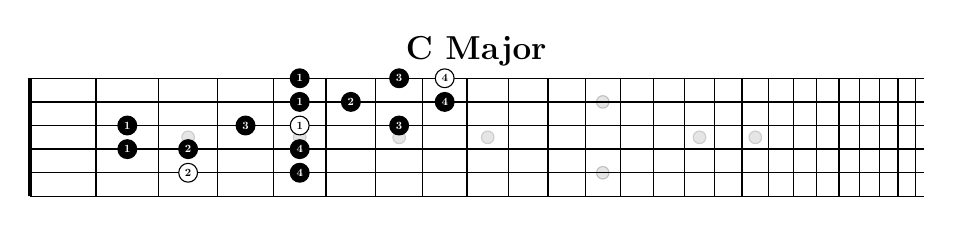
\begin{tikzpicture}[
  ynode/.style={
    draw=red!50,
    circle,
    fill=red!50,
    scale=.35,
    inner sep=1pt,
    minimum size=1.7em}  
]
  
  %%%% Draw the base and set coordinates %%%%
  \begin{scope}[xscale=-15,yscale=.3,line width=.5]

    \xdef\x{1}
    %% Left line
    \draw[line width=1.5] (1,1) -- (1,6);
    \foreach \fret in {1,...,24}{
      %% Set coordinate for each string
      \foreach \str in {1,...,6}{
        \coordinate (\str-\fret) at (0.97193715634*\x,\str);
      }
      %% Set coordinate for the text above
      \coordinate (Top-\fret) at (0.97193715634*\x,7);
      %% Compute the position of the fret
      \pgfmathsetmacro\x{\x * 0.94387431268}
      \xdef\x{\x}
      %% Draw the fret
      \draw (\x,1) -- (\x,6);
    }

    %% Draw each string
    \foreach \str in {1,...,6}{
      \draw (1,\str) -- (0.97153194115*\x,\str);
      \coordinate (start\str) at (1,\str);
    }
  \end{scope}

  %% Draw the fret markers
  \foreach \f in {3,5,7,9,15,17}{
    \draw[black!20,fill=black!10] ($(3-\f)!.5!(4-\f)$) circle (.08);
  }
  \draw[opacity=.20,fill,fill opacity=.10] (2-12) circle (.08) (5-12) circle (.08);

  % example of a chord
  % \node[znode] at (5-4) {\textbf{2}};
  % \node[znode] at (3-5) {\textbf{4}};
  % \draw[zbar] (2-3) -- (5-3);
  \node[above,font=\large\bfseries] at (current bounding box.north) {C Major};
  \node[zroot] at (2-3) {\textbf{2}};
  \node[znode] at (2-5) {\textbf{4}};
  \node[znode] at (3-2) {\textbf{1}};
  \node[znode] at (3-3) {\textbf{2}};
  \node[znode] at (3-5) {\textbf{4}};
  \node[znode] at (4-2) {\textbf{1}};
  \node[znode] at (4-4) {\textbf{3}};
  \node[zroot] at (4-5) {\textbf{1}};
  \node[znode] at (4-7) {\textbf{3}};
  \node[znode] at (5-5) {\textbf{1}};
  \node[znode] at (5-6) {\textbf{2}};
  \node[znode] at (5-8) {\textbf{4}};
  \node[znode] at (6-5) {\textbf{1}};
  \node[znode] at (6-7) {\textbf{3}};
  \node[zroot] at (6-8) {\textbf{4}};
  
\end{tikzpicture}

\vspace{1cm}

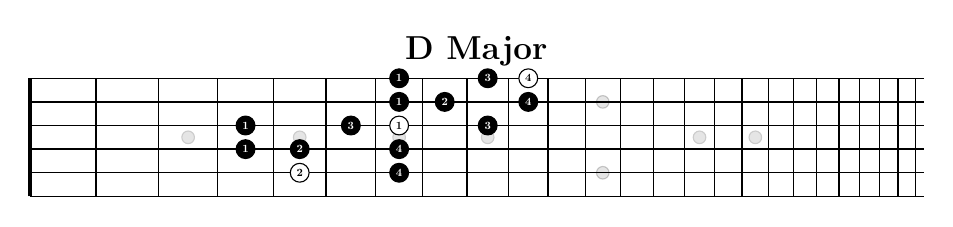
\begin{tikzpicture}[
  ynode/.style={
    draw=red!50,
    circle,
    fill=red!50,
    scale=.35,
    inner sep=1pt,
    minimum size=1.7em}  
]
  
  %%%% Draw the base and set coordinates %%%%
  \begin{scope}[xscale=-15,yscale=.3,line width=.5]

    \xdef\x{1}
    %% Left line
    \draw[line width=1.5] (1,1) -- (1,6);
    \foreach \fret in {1,...,24}{
      %% Set coordinate for each string
      \foreach \str in {1,...,6}{
        \coordinate (\str-\fret) at (0.97193715634*\x,\str);
      }
      %% Set coordinate for the text above
      \coordinate (Top-\fret) at (0.97193715634*\x,7);
      %% Compute the position of the fret
      \pgfmathsetmacro\x{\x * 0.94387431268}
      \xdef\x{\x}
      %% Draw the fret
      \draw (\x,1) -- (\x,6);
    }

    %% Draw each string
    \foreach \str in {1,...,6}{
      \draw (1,\str) -- (0.97153194115*\x,\str);
      \coordinate (start\str) at (1,\str);
    }
  \end{scope}

  %% Draw the fret markers
  \foreach \f in {3,5,7,9,15,17}{
    \draw[black!20,fill=black!10] ($(3-\f)!.5!(4-\f)$) circle (.08);
  }
  \draw[opacity=.20,fill,fill opacity=.10] (2-12) circle (.08) (5-12) circle (.08);

  % example of a chord
  % \node[znode] at (5-4) {\textbf{2}};
  % \node[znode] at (3-5) {\textbf{4}};
  % \draw[zbar] (2-3) -- (5-3);
  \node[above,font=\large\bfseries] at (current bounding box.north) {D Major};
  \node[zroot] at (2-5) {\textbf{2}};
  \node[znode] at (2-7) {\textbf{4}};
  \node[znode] at (3-4) {\textbf{1}};
  \node[znode] at (3-5) {\textbf{2}};
  \node[znode] at (3-7) {\textbf{4}};
  \node[znode] at (4-4) {\textbf{1}};
  \node[znode] at (4-6) {\textbf{3}};
  \node[zroot] at (4-7) {\textbf{1}};
  \node[znode] at (4-9) {\textbf{3}};
  \node[znode] at (5-7) {\textbf{1}};
  \node[znode] at (5-8) {\textbf{2}};
  \node[znode] at (5-10) {\textbf{4}};
  \node[znode] at (6-7) {\textbf{1}};
  \node[znode] at (6-9) {\textbf{3}};
  \node[zroot] at (6-10) {\textbf{4}};
  
\end{tikzpicture}

\end{document}
